\documentclass[12pt,a4paper]{article}
\usepackage[utf8]{inputenc}
\usepackage[T1]{fontenc}
\usepackage[spanish]{babel}
\usepackage{geometry}
\usepackage{graphicx}
\usepackage{listings}
\usepackage{xcolor}
\usepackage{booktabs}
\usepackage{parskip}
\usepackage{fancyhdr}
\usepackage{pdfpages}
\usepackage{microtype}

\geometry{margin=2.5cm}
\setlength{\headheight}{14pt}

\lstset{
    language=Python,
    basicstyle=\ttfamily\footnotesize,
    keywordstyle=\color{blue!70!black}\bfseries,
    stringstyle=\color{red!60!black},
    commentstyle=\color{green!50!black}\itshape,
    backgroundcolor=\color{gray!8},
    frame=single,
    framerule=0.4pt,
    rulecolor=\color{gray!40},
    breaklines=true,
    breakatwhitespace=false,
    columns=flexible,
    showstringspaces=false,
    tabsize=4,
    xleftmargin=0pt,
    xrightmargin=0pt
}

\tolerance=1000
\emergencystretch=1em
\sloppy

\pagestyle{fancy}
\fancyhf{}
\fancyhead[L]{\small UT3T1 -- Sistema Experto}
\fancyhead[R]{\small Documentaci\'on T\'ecnica}
\fancyfoot[C]{\thepage}

\begin{document}

% ============================================================
% PORTADA
% ============================================================
\begin{titlepage}
\centering

\vspace*{2cm}

{\large CIFP Carlos III}

\vspace{0.3cm}

{\normalsize Modelos Big Data}

\vspace{0.5cm}

\rule{\textwidth}{1pt}

\vspace{1.5cm}

{\Huge\bfseries Sistema Experto de\\[0.4cm] Control Clim\'atico de Edificios}

\vspace{1.5cm}

{\Large Documentaci\'on T\'ecnica}

\vspace{0.5cm}

{\large UT3T1 -- Dise\~no e implementaci\'on de un\\sistema experto con Experta}

\vspace{1cm}

\rule{\textwidth}{1pt}

\vspace{2cm}

{\large autor Mart\'inez}

\vfill

{\large Marzo 2026}

\end{titlepage}

\tableofcontents
\newpage

% ============================================================
\section{Dise\~no del sistema}

\subsection{Dominio elegido}

Para este trabajo eleg\'i hacer un sistema de control clim\'atico de un edificio. En la presentaci\'on de la UT3 (cap\'itulo 4) se menciona el control industrial como una de las aplicaciones de los sistemas basados en reglas, y un sistema de climatizaci\'on encaja bien con esa idea: hay datos de sensores, reglas claras de actuaci\'on y situaciones donde el orden de las decisiones importa.

El sistema recibe datos de sensores (temperatura, humedad, CO2, ocupaci\'on) y decide qu\'e hacer: poner calefacci\'on, refrigeraci\'on, ventilaci\'on, etc. Tambi\'en tiene una parte de predicci\'on con series temporales para anticiparse a cambios de temperatura.

Encaja bien con Experta porque:
\begin{itemize}
    \item Los sensores se representan como hechos tipados con \texttt{Field}, igual que \texttt{Persona} y \texttt{Pago} en la sesi\'on 1bis.
    \item Se puede separar el conocimiento (reglas) de los datos (hechos), que es la base de un sistema experto seg\'un la gu\'ia t\'ecnica (cap. 1).
    \item El \texttt{salience} permite dar prioridad a las emergencias sobre el resto de reglas.
\end{itemize}

\subsection{C\'omo funciona}

El sistema sigue el ciclo de ejecuci\'on que describe la gu\'ia t\'ecnica en el cap\'itulo 6 (encadenamiento hacia adelante):

\begin{enumerate}
    \item \texttt{reset()} inicializa la memoria de trabajo y ejecuta los \texttt{@DefFacts}, que en mi caso declaran \texttt{EstadoSistema(modo="normal")}.
    \item Con \texttt{declare()} se a\~naden los hechos de los sensores a la memoria de trabajo.
    \item \texttt{run()} arranca el ciclo de inferencia: el motor busca qu\'e reglas tienen su LHS (antecedente) satisfecho por los hechos actuales, elige la de mayor \texttt{salience}, ejecuta su RHS (consecuente), y repite. Los hechos nuevos que declare el RHS pueden activar m\'as reglas.
\end{enumerate}

\subsection{Hechos del sistema}

Tengo 11 tipos de hechos. Seg\'un la gu\'ia t\'ecnica (cap. 3), cada \texttt{Fact} es una subclase de \texttt{dict} que almacena datos etiquetados. Los divido en tres grupos:

\subsubsection*{Sensores (entrada)}
\begin{itemize}
    \item \texttt{SensorTemperatura}: zona, valor, timestamp
    \item \texttt{SensorHumedad}: zona, valor
    \item \texttt{SensorOcupacion}: zona, personas
    \item \texttt{SensorCO2}: zona, ppm
    \item \texttt{PrediccionTemperatura}: zona, valor\_futuro, horizonte\_min (viene del modelo predictivo)
\end{itemize}

\subsubsection*{Hechos derivados (los generan las reglas)}
\begin{itemize}
    \item \texttt{NivelConfort}: zona, nivel (frio/optimo/caluroso)
    \item \texttt{NivelCalidadAire}: zona, nivel (bueno/regular/malo)
    \item \texttt{RiesgoEnergetico}: zona, nivel
\end{itemize}

\subsubsection*{Salidas}
\begin{itemize}
    \item \texttt{AccionControl}: zona, sistema, accion, intensidad
    \item \texttt{Alerta}: zona, tipo, mensaje, prioridad
    \item \texttt{EstadoSistema}: modo (normal/ahorro/emergencia)
\end{itemize}

\subsection{Cadena de inferencia multinivel}

Las reglas van por niveles, cada nivel usa lo que ha generado el anterior:

\begin{lstlisting}[language={},basicstyle=\ttfamily\footnotesize]
Nivel 0: Datos de sensores + PrediccionTemperatura
    |
    | [salience=100] Emergencias
    | temp >45 o <0, CO2 >5000 -> Alerta
    v
Nivel 1: NivelConfort, NivelCalidadAire
    |
    | [salience=50] Clasificacion
    | temp -> frio/optimo/caluroso
    | CO2 -> bueno/regular/malo
    v
Nivel 2: RiesgoEnergetico
    |
    | [salience=50] Ocupacion alta + temp mala -> riesgo
    v
Nivel 3: AccionControl, Alerta
    |
    | [salience=20] Control
    | confort + ocupacion -> calef/refrig/ventil
    v
Nivel 4: Ajustes
    |
    | [salience=10] Optimizacion
    | conflicto energia -> bajar intensidad
\end{lstlisting}

Cuando empec\'e a hacer las reglas no usaba salience y no me funcionaba porque las reglas de control se ejecutaban antes de que existieran los hechos de clasificaci\'on. Separarlo en niveles solucion\'o el problema.

% ============================================================
\newpage
\section{Reglas y comportamiento}

\subsection{Reglas implementadas}

El sistema tiene 17 reglas repartidas en 4 niveles de prioridad.

\subsubsection*{Emergencias (salience=100) -- 2 reglas}
\begin{itemize}
    \item \texttt{emergencia\_temp}: salta si la temperatura pasa de 45 o baja de 0. Usa \texttt{P(lambda t: t > 45 or t < 0)}.
    \item \texttt{emergencia\_co2}: salta si el CO2 pasa de 5000~ppm.
\end{itemize}

\subsubsection*{Clasificaci\'on (salience=50) -- 7 reglas}
\begin{itemize}
    \item 3 para temperatura: frio (<19), optimo (19--26), caluroso (>26). Llevan \texttt{NOT(Alerta(...))} para no clasificar si hay emergencia.
    \item 3 para calidad del aire: bueno ($\leq$400), regular (401--1000), malo (1001--5000).
    \item 1 de riesgo energ\'etico: m\'as de 30 personas y confort no \'optimo. Usa \texttt{OR()} para pillar frio o caluroso.
\end{itemize}

\subsubsection*{Control (salience=20) -- 5 reglas}
\begin{itemize}
    \item Calefacci\'on si frio + hay gente.
    \item Refrigeraci\'on si caluroso + hay gente.
    \item Ventilaci\'on forzada si aire malo.
    \item Modo ahorro si no hay nadie y temp \'optima.
    \item Pre-enfriamiento si la predicci\'on dice que va a subir de 28\textdegree C (usa series temporales).
\end{itemize}

Todas llevan \texttt{NOT()} para no duplicar acciones. Al principio no lo pon\'ia y me generaba la misma acci\'on varias veces.

\subsubsection*{Optimizaci\'on (salience=10) -- 3 reglas}
\begin{itemize}
    \item Si hay refrigeraci\'on alta + riesgo energ\'etico, baja a moderada con \texttt{modify()}.
    \item Si caluroso + humedad >70\%, activa deshumidificador.
    \item Ventilaci\'on preventiva si hay bastante gente y aire regular.
\end{itemize}

\subsection{Operadores que he usado}

\begin{itemize}
    \item \texttt{P(lambda)}: para condiciones num\'ericas, como \texttt{P(lambda t: t > 45 or t < 0)}.
    \item \texttt{L("valor")}: para comparar con un valor exacto.
    \item \texttt{NOT()}: para comprobar que un hecho no existe. Lo uso bastante para evitar duplicados.
    \item \texttt{OR()}: para agrupar condiciones. La uso en la regla de riesgo energ\'etico.
    \item \texttt{AS.accion << AccionControl(...)}: captura el hecho para poder modificarlo despu\'es con \texttt{modify()}.
    \item \texttt{MATCH.zona}: enlaza el campo zona a una variable para usarla luego.
\end{itemize}

% ============================================================
\newpage
\section{An\'alisis de variaci\'on}

\subsection{Variaci\'on de temperatura}

Hice un barrido de $-5$\textdegree C a $54$\textdegree C con CO2 fijo a 500 y 10 personas para ver c\'omo reacciona el sistema:

\begin{table}[h]
\centering
\begin{tabular}{llll}
\toprule
\textbf{Rango} & \textbf{Confort} & \textbf{Acci\'on} & \textbf{Emergencia} \\
\midrule
T < 0\textdegree C & no clasifica & parada & S\'I \\
0--18\textdegree C & frio & calefacci\'on & NO \\
19--26\textdegree C & \'optimo & ninguna & NO \\
27--44\textdegree C & caluroso & refrigeraci\'on & NO \\
T > 45\textdegree C & no clasifica & parada & S\'I \\
\bottomrule
\end{tabular}
\caption{Respuesta seg\'un temperatura}
\end{table}

Las transiciones salen limpias, no se solapan los rangos. En emergencias no se clasifican porque las reglas de clasificaci\'on llevan \texttt{NOT(Alerta(...))}.

\subsection{Variaci\'on del CO2}

\begin{table}[h]
\centering
\begin{tabular}{llll}
\toprule
\textbf{Rango} & \textbf{Calidad} & \textbf{Ventilaci\'on} & \textbf{Emergencia} \\
\midrule
$\leq$ 400 ppm & bueno & NO & NO \\
401--1000 ppm & regular & si >15 personas & NO \\
1001--5000 ppm & malo & S\'I (forzada) & NO \\
> 5000 ppm & N/A & S\'I (emergencia) & S\'I \\
\bottomrule
\end{tabular}
\caption{Respuesta seg\'un CO2}
\end{table}

La ventilaci\'on preventiva con aire regular es un caso donde se combinan datos de CO2 y de ocupaci\'on para decidir.

\subsection{Efecto de la ocupaci\'on}

\begin{itemize}
    \item 0 personas: modo ahorro (si temp \'optima)
    \item > 0 personas: se activan calefacci\'on/refrigeraci\'on
    \item > 15 personas: ventilaci\'on preventiva (con aire regular)
    \item > 30 personas: riesgo energ\'etico (si temp no \'optima)
\end{itemize}

\subsection{Efecto de la predicci\'on}

\begin{table}[h]
\centering
\begin{tabular}{lll}
\toprule
\textbf{Predicci\'on (30 min)} & \textbf{Temp actual} & \textbf{Acci\'on} \\
\midrule
< 28\textdegree C & \'optima (22\textdegree C) & ninguna \\
$\geq$ 28\textdegree C & \'optima (22\textdegree C) & pre-enfriamiento \\
$\geq$ 28\textdegree C & calurosa (30\textdegree C) & refrigeraci\'on \\
\bottomrule
\end{tabular}
\caption{Efecto de la predicci\'on}
\end{table}

El pre-enfriamiento solo salta cuando ahora est\'a bien pero se espera que suba. Si ya hace calor, la refrigeraci\'on normal tiene m\'as prioridad.

% ============================================================
\newpage
\section{Estrategias de control}

\subsection{Niveles de prioridad}

Uso 4 valores de \texttt{salience}:

\textbf{salience=100 -- Emergencias:} Lo primero es la seguridad. Si la temperatura es peligrosa o el CO2 es t\'oxico, se genera una alerta y se bloquean las reglas de clasificaci\'on para que no intente climatizar una zona que habr\'ia que evacuar.

\textbf{salience=50 -- Clasificaci\'on:} Convierte los datos de sensores en categor\'ias (frio, caluroso, aire malo...). Si esto no va antes que el control, las reglas de control no encuentran los hechos que necesitan y no hacen nada. Es lo que me pasaba al principio.

\textbf{salience=20 -- Control:} Genera acciones concretas a partir de las clasificaciones.

\textbf{salience=10 -- Optimizaci\'on:} Ajusta acciones cuando hay conflictos, por ejemplo bajar la intensidad si el gasto es alto.

\subsection{Conflicto confort vs energ\'ia}

Es el caso m\'as interesante. Cuando hace calor y hay mucha gente pasan estas cosas en orden:

\begin{enumerate}
    \item Se clasifica como caluroso (salience=50)
    \item Se detecta riesgo energ\'etico porque hay >30 personas con temp no \'optima (salience=50)
    \item Se activa refrigeraci\'on alta (salience=20)
    \item La regla de optimizaci\'on ve que hay refrigeraci\'on alta + riesgo energ\'etico y baja la intensidad a moderada con \texttt{modify()} (salience=10)
\end{enumerate}

Para hacer el \texttt{modify()} uso \texttt{AS.accion << AccionControl(...)} para capturar el hecho y luego \texttt{self.modify(accion, intensidad="moderada")}. Es parecido al ejemplo de pr\'estamos de la sesi\'on 1bis.

% ============================================================
\newpage
\section{Series temporales}

\subsection{Datos y modelo}

Genero datos falsos de temperatura para 7 d\'ias (168 registros, uno por hora). Los datos simulan un ciclo d\'ia/noche, efecto fin de semana (2 grados menos), tendencia ascendente y ruido aleatorio.

El modelo es una regresi\'on polinomial de grado 3 con scikit-learn. Como features uso:
\begin{itemize}
    \item \texttt{hora\_sin} y \texttt{hora\_cos}: para codificar la hora de forma c\'iclica (que las 23h est\'en cerca de las 0h).
    \item \texttt{dia\_semana}: n\'umero del d\'ia.
    \item \texttt{es\_finde}: 1 si es s\'abado o domingo.
\end{itemize}

\subsection{C\'omo se integra con el experto}

La predicci\'on se mete como un hecho m\'as antes de ejecutar el motor:

\begin{lstlisting}
temp_predicha = predecir_temp(modelo, hora + 0.5, dia)
engine.declare(PrediccionTemperatura(
    zona="oficina",
    valor_futuro=temp_predicha,
    horizonte_min=30
))
\end{lstlisting}

La regla \texttt{control\_predictivo} se activa si la predicci\'on pasa de 28\textdegree C, la temperatura actual es \'optima y hay gente en la zona. As\'i el sistema puede actuar 30 minutos antes de que suba la temperatura.

% ============================================================
\newpage
\section{Plan de pruebas}

\subsection{Casos de prueba}

Hice 12 tests para cubrir distintas situaciones:

\begin{table}[h]
\centering
\small
\begin{tabular}{lllp{3.8cm}l}
\toprule
\textbf{ID} & \textbf{Tipo} & \textbf{Prueba} & \textbf{Entrada} & \textbf{Esperado} \\
\midrule
T01 & Normal & Calefacci\'on & Temp=15, Ocup=5 & calefaccion \\
T02 & Normal & Refrigeraci\'on & Temp=32, Ocup=3 & refrigeracion \\
T03 & Normal & Ventilaci\'on & CO2=1500 & ventilacion \\
T04 & Normal & Sin acci\'on & T=22, CO2=400, Oc=5 & optimo \\
T05 & Multi & Cadena & Temp=15, Ocup=3 & frio+calef \\
T06 & Multi & Riesgo energ. & T=30, Ocup=50 & refrig. mod. \\
T07 & Multi & Predicci\'on & T=24, Pred=30 & pre-enfr. \\
T08 & Prior. & Emergencia & Temp=50 & alerta cr\'it. \\
T09 & Prior. & Ahorro & Temp=22, Ocup=0 & modo ahorro \\
T10 & L\'imite & Umbral 19 & Temp=19.0 & \'optimo \\
T11 & Robust. & Sin temp & Solo Ocup=5 & sin acciones \\
T12 & Robust. & Dos zonas & A:fria, B:caliente & calef+refrig \\
\bottomrule
\end{tabular}
\caption{Casos de prueba}
\end{table}

\subsection{Qu\'e cubre cada grupo}

\begin{itemize}
    \item T01--T04: operaci\'on normal, que las reglas b\'asicas funcionen.
    \item T05--T07: inferencia multinivel. T05 comprueba la cadena sensor-confort-acci\'on, T06 que el riesgo modifica la intensidad, T07 que la predicci\'on activa el pre-enfriamiento.
    \item T08--T09: que el salience funciona bien.
    \item T10: caso l\'imite, que 19.0 se clasifica como \'optimo.
    \item T11--T12: robustez. T11 que sin datos de temperatura no falla, T12 que dos zonas opuestas se manejan por separado.
\end{itemize}

Los 12 pasan correctamente.

% ============================================================
\newpage
\section*{Anexo: C\'odigo fuente (Notebook)}

A continuaci\'on va el PDF exportado desde Jupyter con todo el c\'odigo y sus salidas.

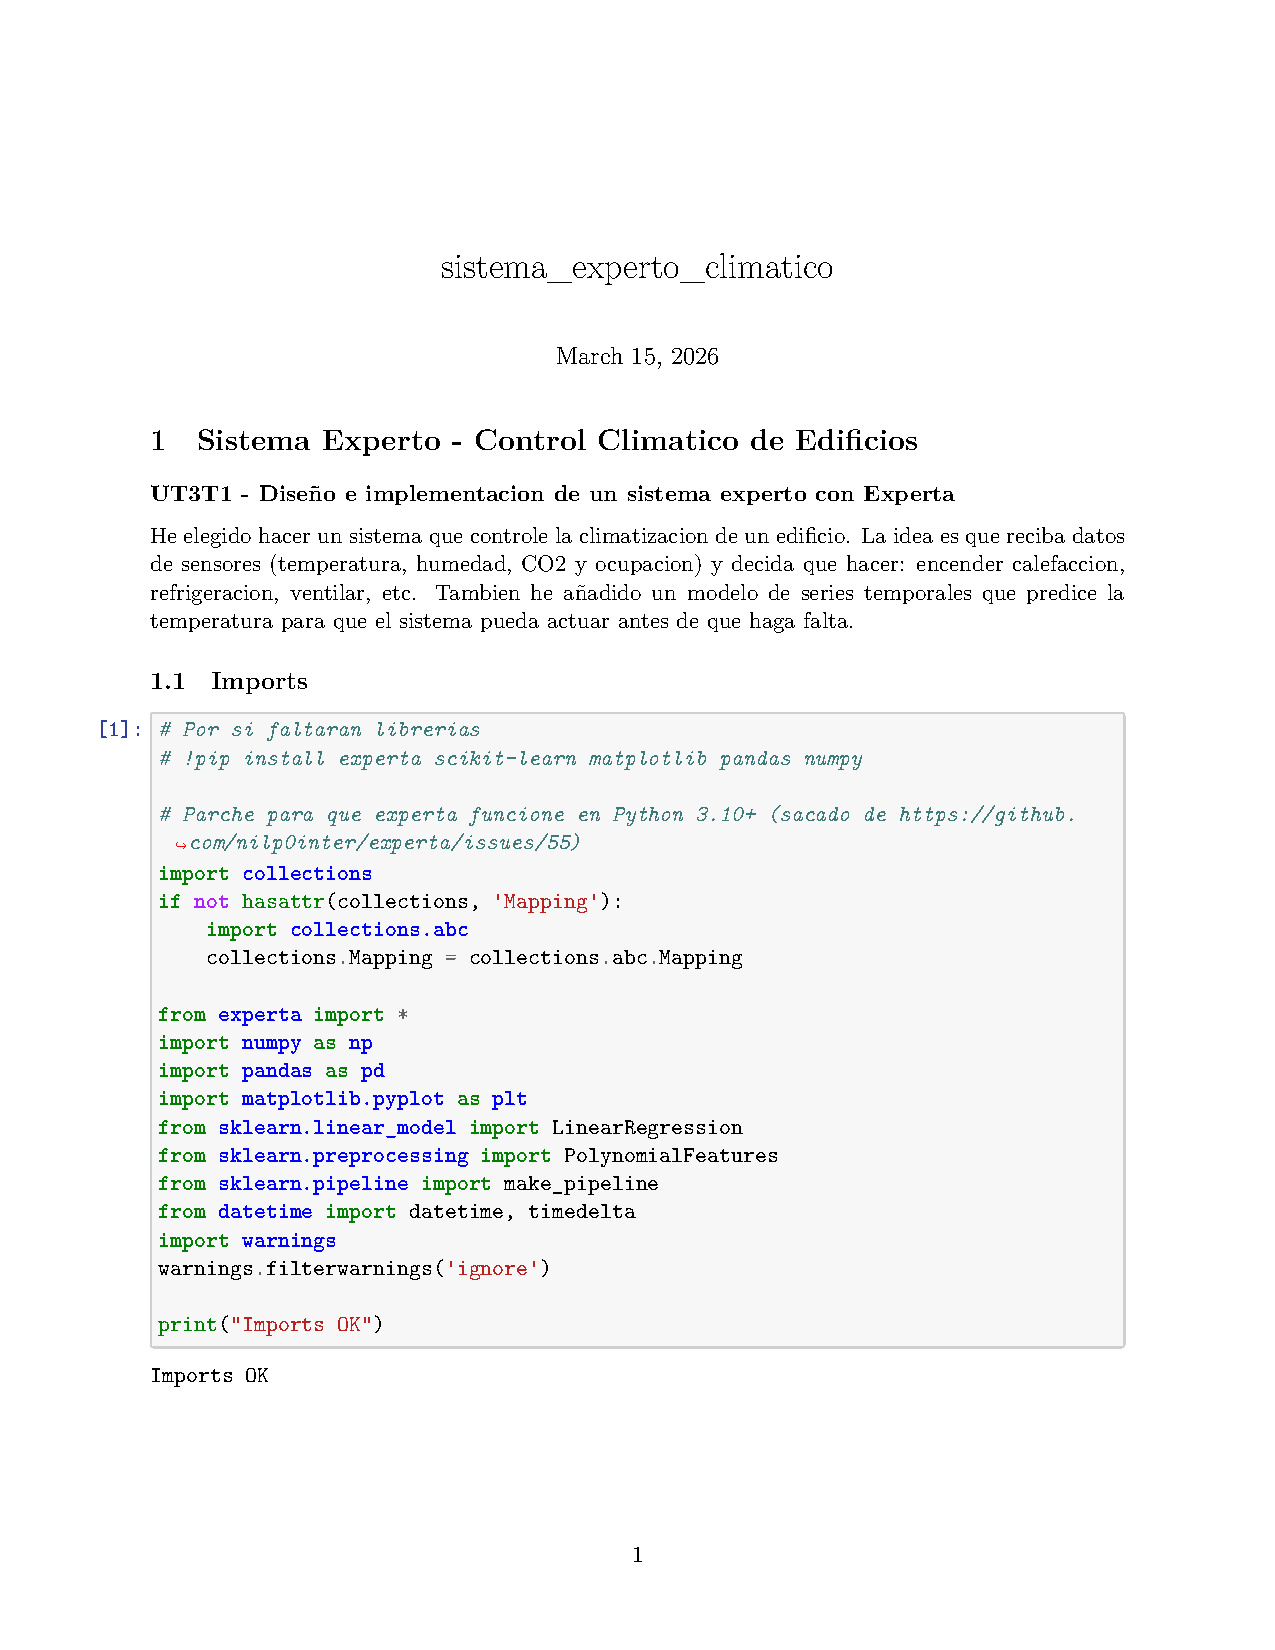
\includepdf[pages=-,pagecommand={\thispagestyle{fancy}}]{sistema_experto_climatico.pdf}

\end{document}
